\chapter{Physical Design}
\label{physical_design}

% Below is shown how you can insert a figure. If you give a label to the figure, you can refer to the figure using \ref{figure_label} as shown above. 
	\begin{figure}[ht]
	\centering
	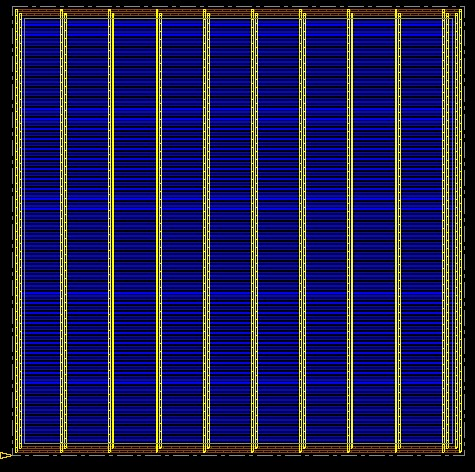
\includegraphics[width=\textwidth]{chapters/figures/4.horizontal_lines.jpg} 
	\caption{Power grid distribution}
	\label{fig:power_distribution}  % here is the figure label
	\end{figure}

This is the final step, in which the layout of our DLX design can be generated, using the \textbf{Innovus} tool, provided by Cadence.
The entire procedure is composed of various steps, from Floorplanning to Cell Placing and signal Routing.

To start creating the floorplan, Innovus needs a verilog post-synthesis netlist, a \textit{.lef} file that has references to the library of cells and other data which is
provided in the project files. In this step the area dedicated to the chip core is computed, along with the power supply rings around it.
%% put figure
Next, the power rings for \textit{Vdd} and \textit{GND} are inserted in the model and on the layout corner, the vias to connect the metal layer are placed as well. To avoid congestion, M9 and M10 metals are chosen for the rings.
The rings are then connected using vertical stripes and horizontal lines, to better distribute power into the center of the chip.
Power Grid Placement is shown in Figure \ref{fig:power_distribution}.

\begin{figure}[ht]
	\centering
	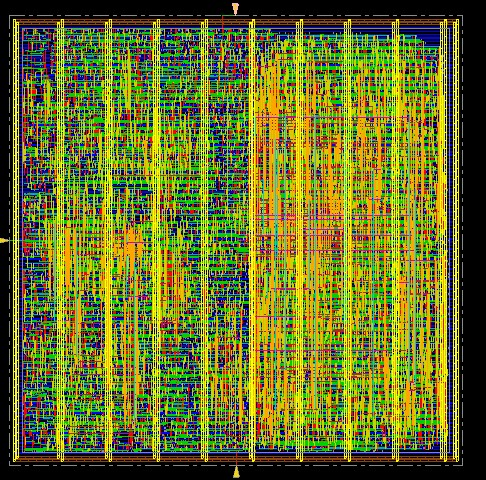
\includegraphics[width=\textwidth]{chapters/figures/7.Post_CTS_optimization.jpg} 
	\caption{Post CTS Optimization}
	\label{fig:CTS_OPT}  % here is the figure label
	\end{figure}

\section{Placement and Routing}
In the Placement phase, the cells are placed, along with I/O pins. Post CTS (Clock-Tree-Synthesis) optimization is performed before routing.
The result is shown in Figure \ref{fig:CTS_OPT}.
Before the routing phase, it is important to complete the placement filling free spaces in the layout with \textit{Filler Cells}, to maintain the continuity of the N+ and P+ wells.

The final step is the \textbf{Post routing optimization}, in which the design is optimized in order to achieve the timing constraints.
Now the design is complete and a final verification can be performed to see if there are violations with respect to design rules and connectivity.

\begin{figure}[ht]
	\centering
	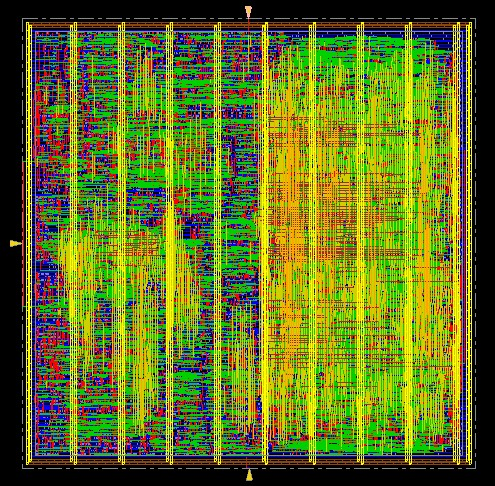
\includegraphics[width=\textwidth]{chapters/figures/9.Post_PostRouteOPT.jpg} 
	\caption{Final layout}
	\label{fig:final_design}  % here is the figure label
	\end{figure}

The final layout is shown in \ref{fig:final_design}









